\documentclass[pdf]{beamer}
\usetheme{Singapore}
%\usetheme{Warsaw}
%\usetheme{PaloAlto}


\usepackage{enumerate}
\usepackage{hyperref}
\usepackage{graphicx}
\usepackage{color}
\usepackage{amsmath}
\usepackage{amsfonts}
\usepackage{amssymb}
\definecolor{olivegreen}{RGB}{30,100,49}

%\beamertemplatenavigationsymbolsempty
%\setbeamercolor{footline}{fg=blue}
\setbeamertemplate{footline}[frame number]
\setbeamertemplate{blocks}[rounded][shadow=false]
\setbeamercolor{block title}{fg=structure,bg=white}
\setbeamertemplate{background canvas}[vertical shading][bottom=red!1,top=blue!25]
%\usepackage{default}

\title{An Introduction to Bucket Sort}
\author{Amlan Saha\\Dhiman Goswami}
\institute{Bangladesh University of Engineering and Technology\\Dhaka, Bangladesh}
\date{\today}

\begin{document}

\begin{frame}
\titlepage
\end{frame}

\begin{frame}
	\frametitle{Let's see a problem}
		\pause
		A batsman scores the following runs in a tournament.
		\pause
		\begin{table}[h]
			\centering
			\begin{tabular}{|c|c|c|c|c|c|c|c|}
				\hline
				29 & 25 & 3 & 49 & 9 & 37 & 21 & 43\\
				\hline
			\end{tabular}
		\end{table}
		\pause
		\textbf{Sort the array of numbers.}		
\end{frame}

\begin{frame}
	\frametitle{Possible Solution}
	%What could be our approach to solve this problem?\\
	\pause
	We can use some commonly used algorithms here. Like:
	\pause
	\begin{itemize}
		\item Insertion Sort
		\pause
		\item Bubble Sort
		\pause
		\item Merge Sort
		\pause
		\item Quick Sort
		\pause
		\item etc.
	\end{itemize}
\end{frame}

\begin{frame}
	%\frametitle{Possible Solution}
	\begin{block}{
		\color{red}
		\textit{But wait!!!}}
	\end{block}
	\pause
	\begin{block}{
		\color{red}
		\textit{All those algorithms take at least $n lg(n)$ time to sort the array.}}
	\end{block}
	\pause
	\begin{block}{
		\color{blue}
		\textit{Can we sort in linear time?}}
	\end{block}

	\pause
	\begin{block}{
		\color{olivegreen}\textit{Yes, we can :)}}
	\end{block}	
\end{frame}


\begin{frame}
	\frametitle{BUCKET SORT!!!}
	\begin{columns}
		\column{0.5\textwidth}
		\begin{block}{
			\color{black}\textit{Bucket sorting is a linear time algoritm of sorting}}
		\end{block}
		\pause
		\column{0.5\textwidth}
		\begin{figure}
			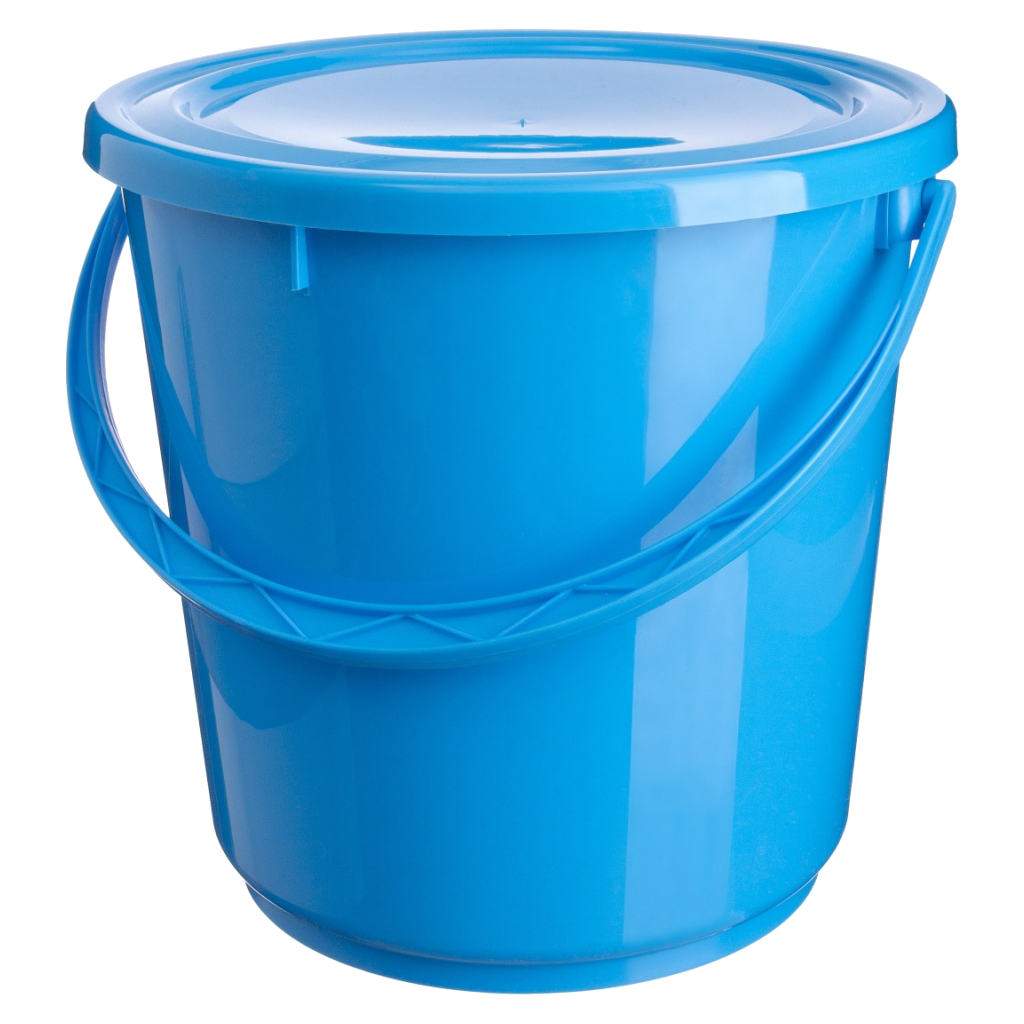
\includegraphics[scale=0.1]{Figure/bucket.png}
		%\caption{Bucket!!!}
		\end{figure}
	\end{columns}

%\frametitle{Pictures}
\end{frame}


\begin{frame}
	\textbf{Assumptions:}
	\begin{itemize}
		\pause
		\item inputs are in a small range.
		\pause
		\item inputs are distributed uniformly over the range.
	\end{itemize}
\end{frame}

\begin{frame}
	\frametitle{}
\end{frame}

\begin{frame}
	\frametitle{Back to our problem.}
		\begin{table}[h]
			\centering
			\begin{tabular}{|c|c|c|c|c|c|c|c|c|}
				\hline
				Index & 0 & 1 & 2 & 3 & 4 & 5 & 6 & 7 \\
				\hline
				Value & 29 & 25 & 3 & 49 & 9 & 37 & 21 & 43\\
				\hline
			\end{tabular}
		\end{table}
		\pause
		Here, we assume
		\begin{itemize}
			\item Array size: 8
			\item Input range: 0-49
			\item Let's insert these numbers into 5 buckets.
		\end{itemize}
\end{frame}

\begin{frame}
	\frametitle{Sorting...}
	\begin{figure}
		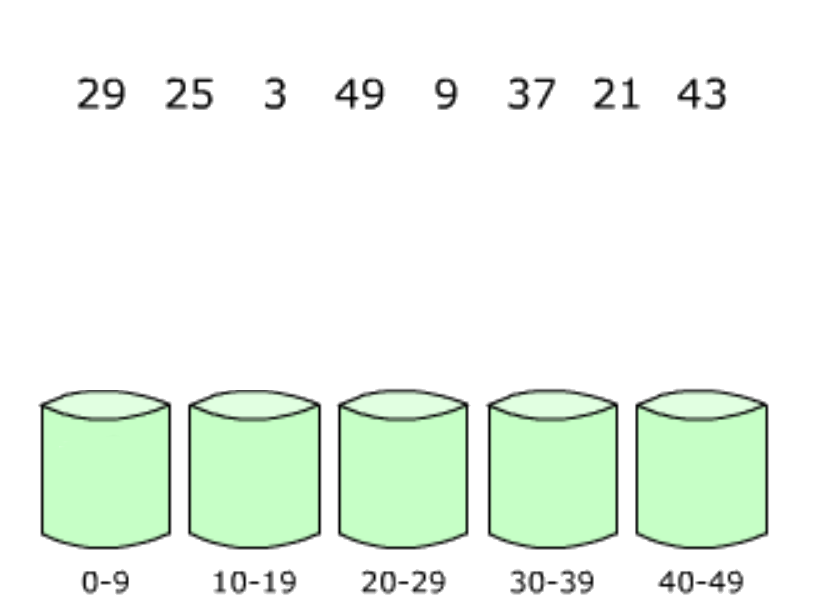
\includegraphics[scale=.3]{Figure/0.png}
	\end{figure}	
\end{frame}

\begin{frame}
	\frametitle{Sorting...}
	\begin{figure}
		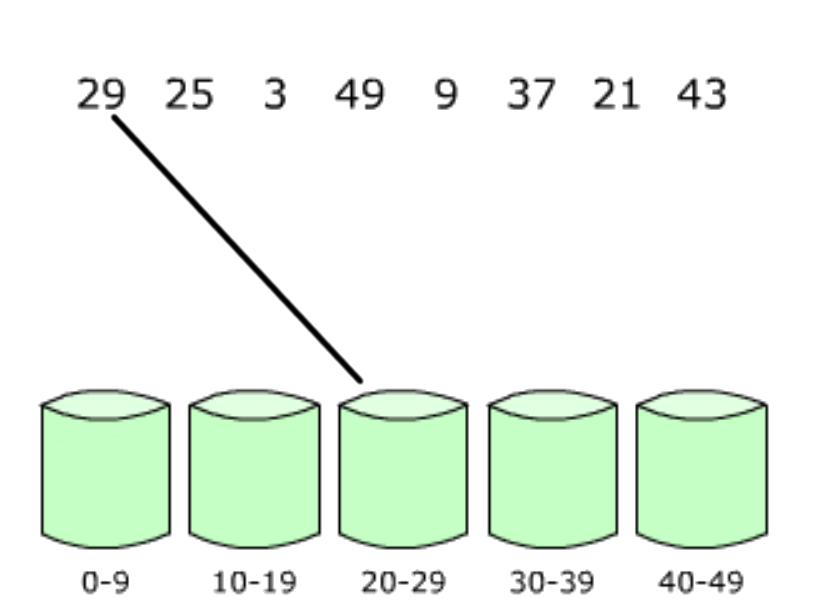
\includegraphics[scale=.3]{Figure/1.png}
	\end{figure}	
\end{frame}

\begin{frame}
	\frametitle{Sorting...}
	\begin{figure}
		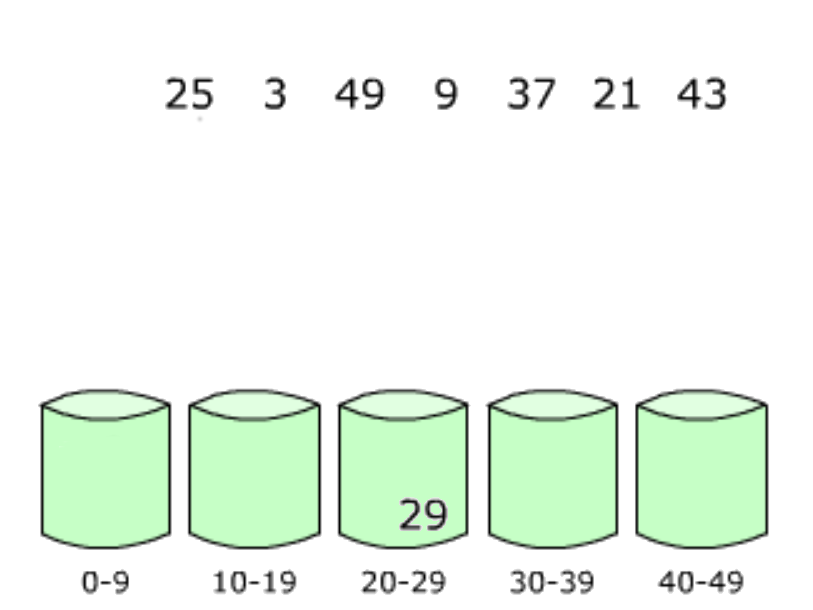
\includegraphics[scale=.3]{Figure/2.png}
	\end{figure}	
\end{frame}

\begin{frame}
	\frametitle{Sorting...}
	\begin{figure}
		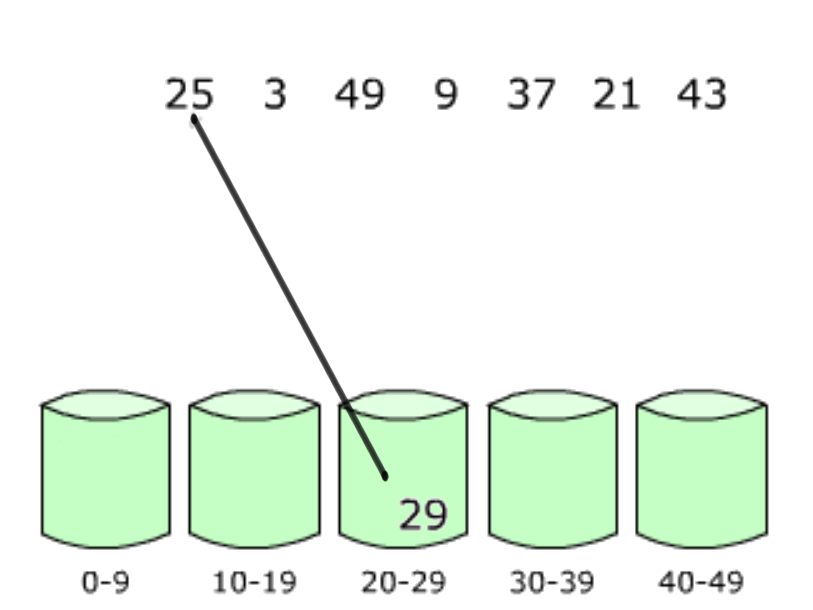
\includegraphics[scale=.3]{Figure/3.png}
	\end{figure}	
\end{frame}

\begin{frame}
	\frametitle{Sorting...}
	\begin{figure}
		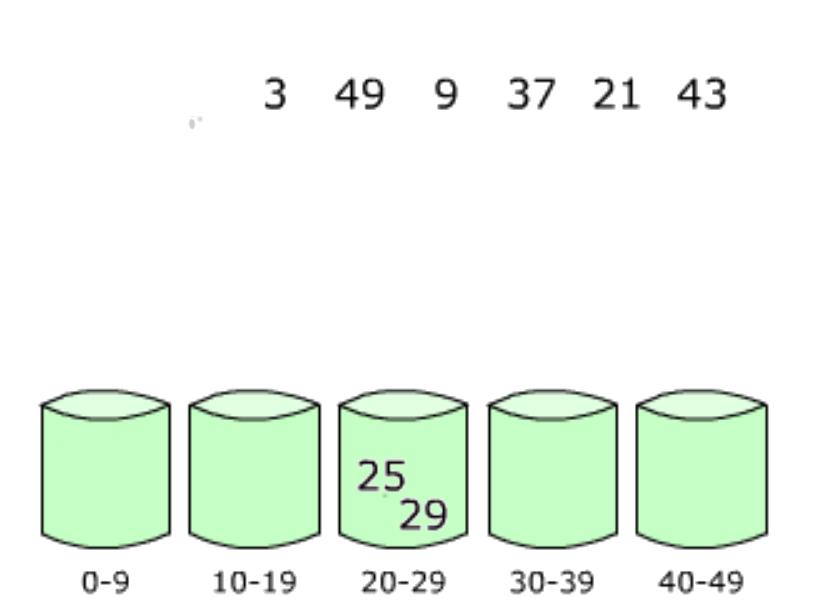
\includegraphics[scale=.3]{Figure/4.png}
	\end{figure}	
\end{frame}

\begin{frame}
	\frametitle{Sorting...}
	\begin{figure}
		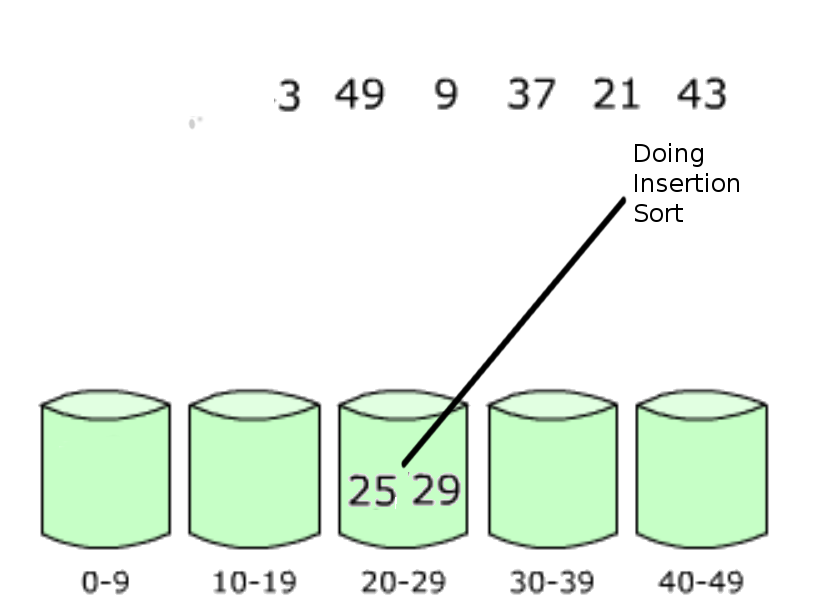
\includegraphics[scale=.3]{Figure/4-i.png}
	\end{figure}	
\end{frame}

\begin{frame}
	\frametitle{Sorting...}
	\begin{figure}
		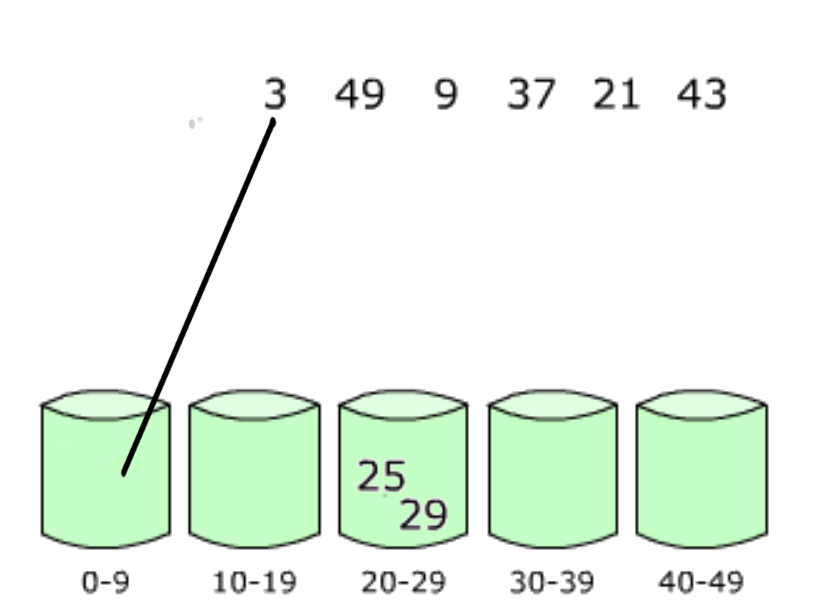
\includegraphics[scale=.3]{Figure/5.png}
	\end{figure}	
\end{frame}

\begin{frame}
	\frametitle{Sorting...}
	\begin{figure}
		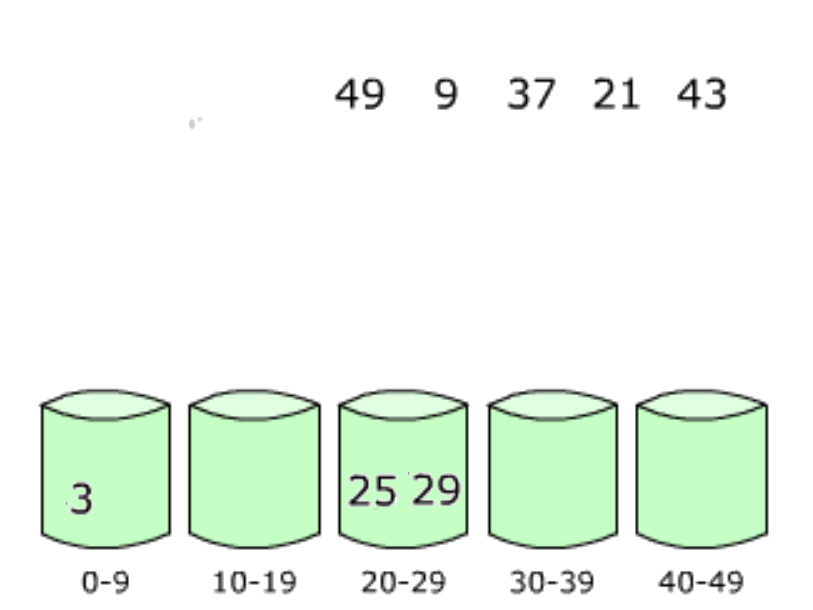
\includegraphics[scale=.3]{Figure/6.png}
	\end{figure}	
\end{frame}

\begin{frame}
	\frametitle{Sorting...}
	\begin{figure}
		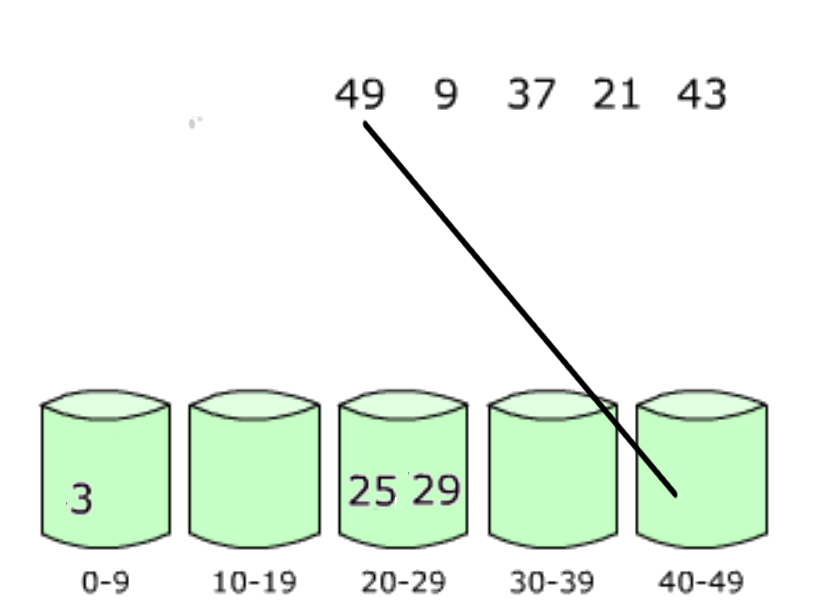
\includegraphics[scale=.3]{Figure/7.png}
	\end{figure}	
\end{frame}

\begin{frame}
	\frametitle{Sorting...}
	\begin{figure}
		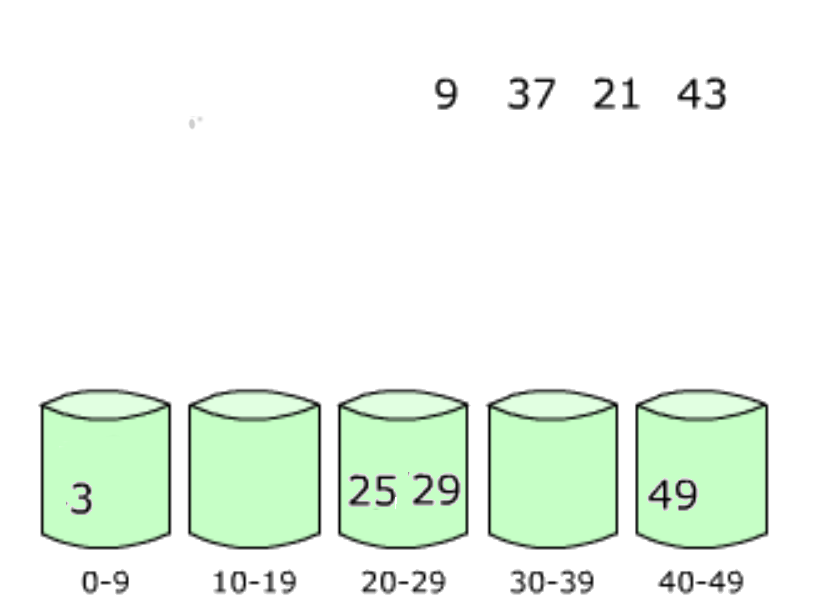
\includegraphics[scale=.3]{Figure/8.png}
	\end{figure}	
\end{frame}

\begin{frame}
	\frametitle{Sorting...}
	\begin{figure}
		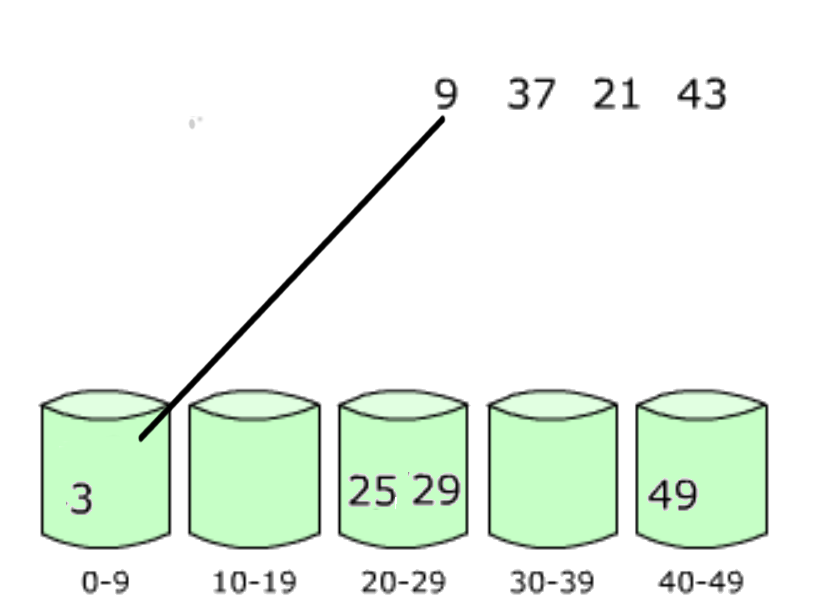
\includegraphics[scale=.3]{Figure/9.png}
	\end{figure}	
\end{frame}

\begin{frame}
	\frametitle{Sorting...}
	\begin{figure}
		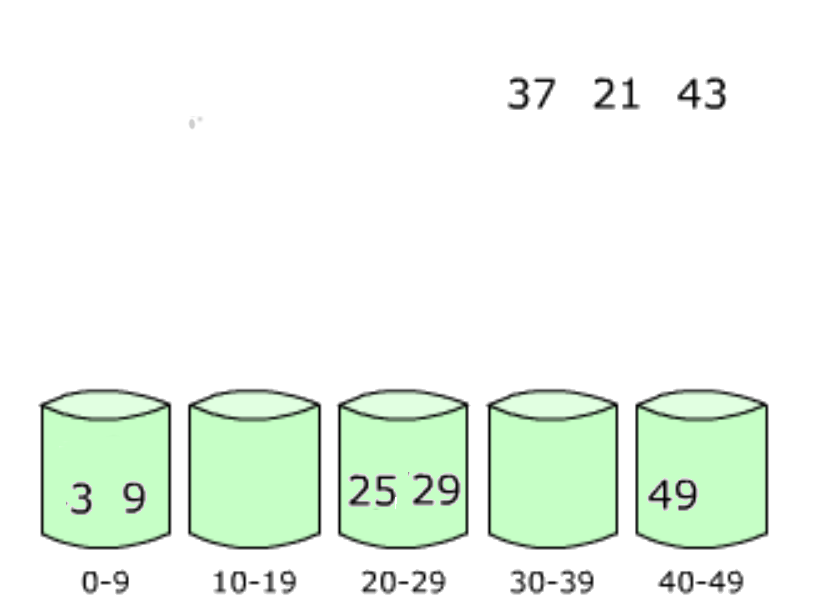
\includegraphics[scale=.3]{Figure/10.png}
	\end{figure}	
\end{frame}

\begin{frame}
	\frametitle{Sorting...}
	\begin{figure}
		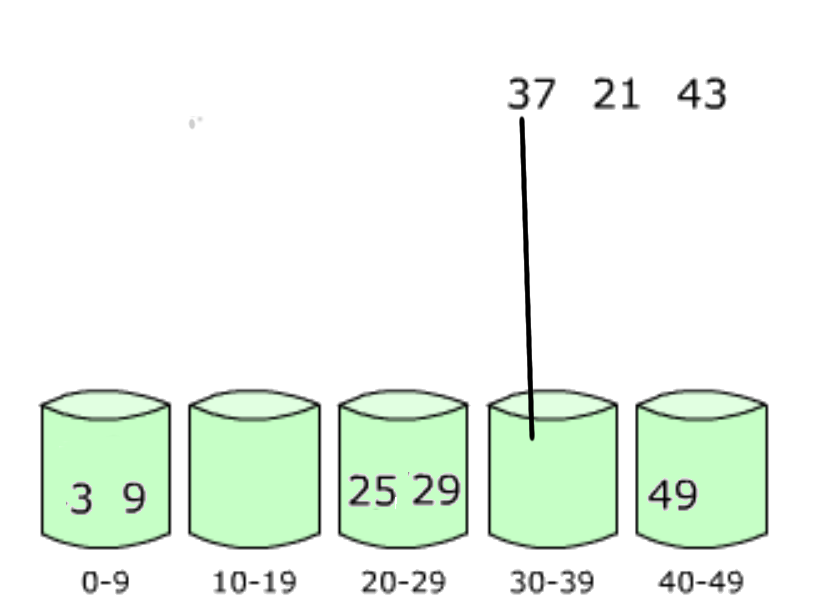
\includegraphics[scale=.3]{Figure/11.png}
	\end{figure}	
\end{frame}

\begin{frame}
	\frametitle{Sorting...}
	\begin{figure}
		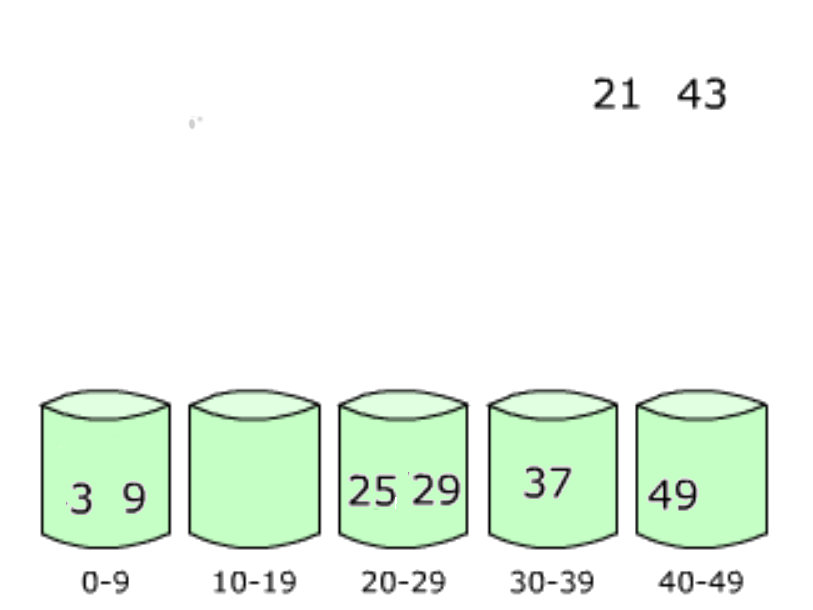
\includegraphics[scale=.3]{Figure/12.png}
	\end{figure}	
\end{frame}

\begin{frame}
	\frametitle{Sorting...}
	\begin{figure}
		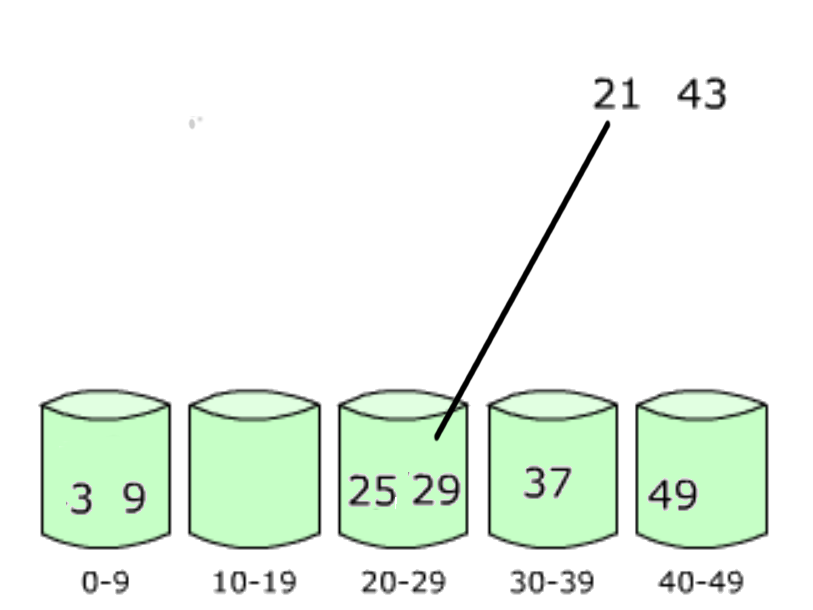
\includegraphics[scale=.3]{Figure/13.png}
	\end{figure}	
\end{frame}

\begin{frame}
	\frametitle{Sorting...}
	\begin{figure}
		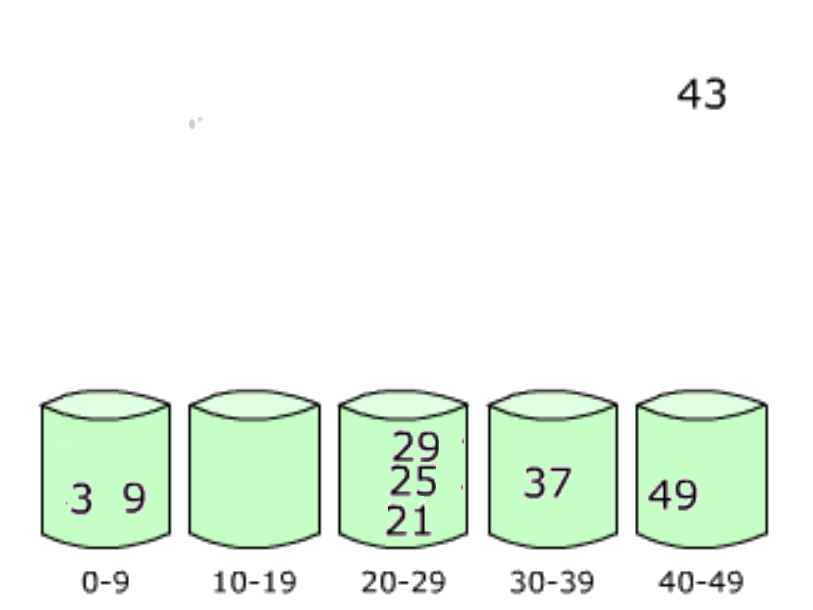
\includegraphics[scale=.3]{Figure/14.png}
	\end{figure}	
\end{frame}
\begin{frame}
	\frametitle{Sorting...}
	\begin{figure}
		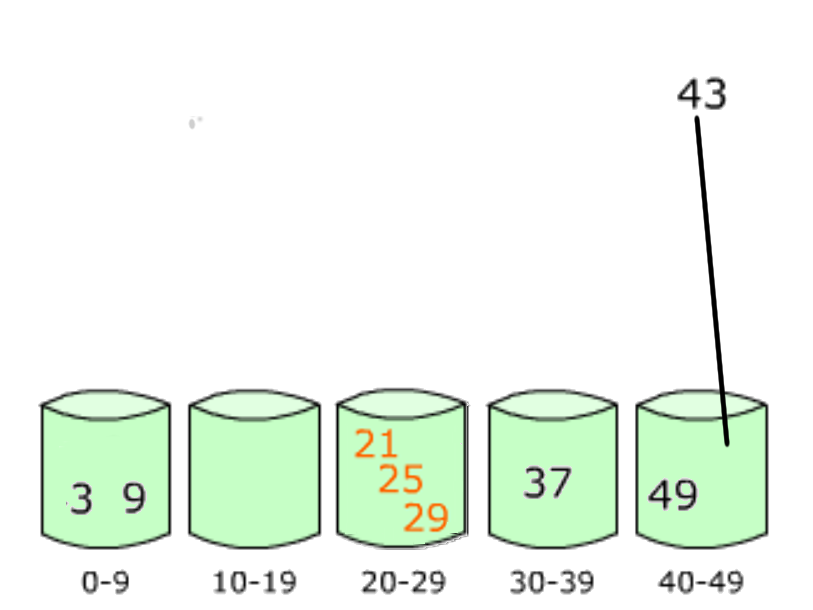
\includegraphics[scale=.3]{Figure/15.png}
	\end{figure}	
\end{frame}
\begin{frame}
	\frametitle{Sorting...}
	\begin{figure}
		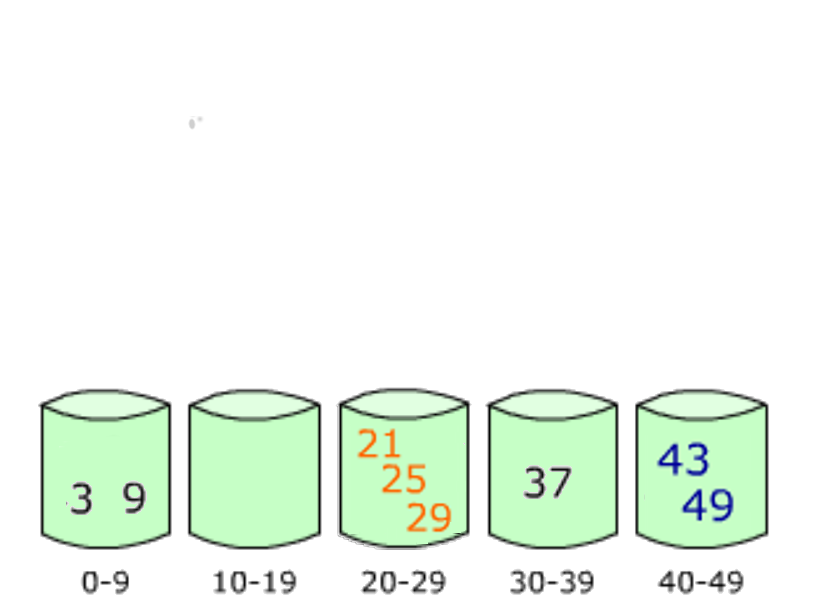
\includegraphics[scale=.3]{Figure/16.png}
	\end{figure}	
\end{frame}
\begin{frame}
	\frametitle{Sorting...}
	\begin{figure}
		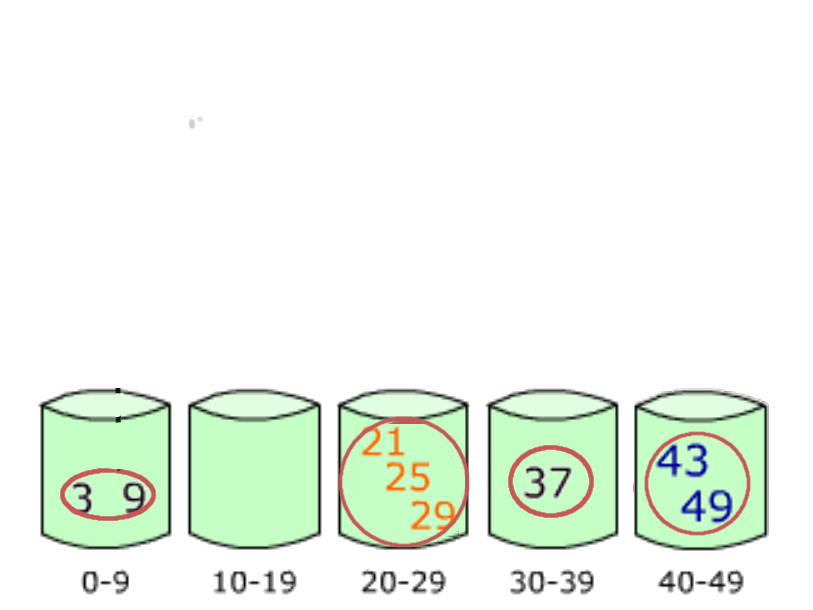
\includegraphics[scale=.3]{Figure/17.png}
	\end{figure}	
\end{frame}
\begin{frame}
	\frametitle{Sorting...}
	\begin{figure}
		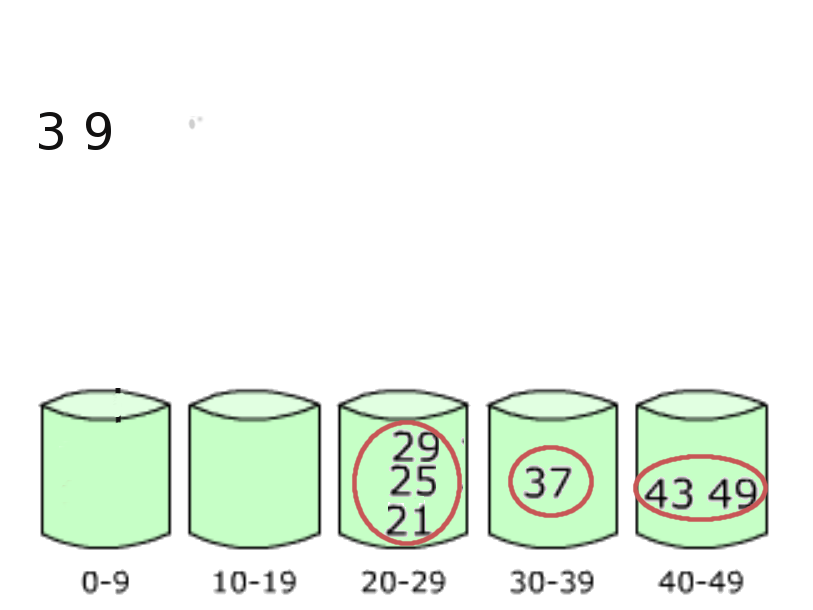
\includegraphics[scale=.3]{Figure/18.png}
	\end{figure}	
\end{frame}
\begin{frame}
	\frametitle{Sorting...}
	\begin{figure}
		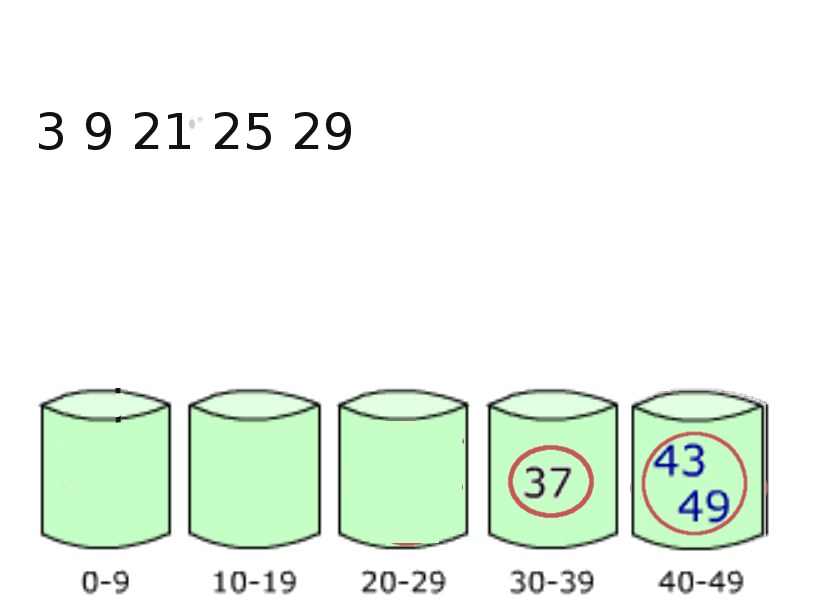
\includegraphics[scale=.3]{Figure/19.png}
	\end{figure}	
\end{frame}
\begin{frame}
	\frametitle{Sorting...}
	\begin{figure}
		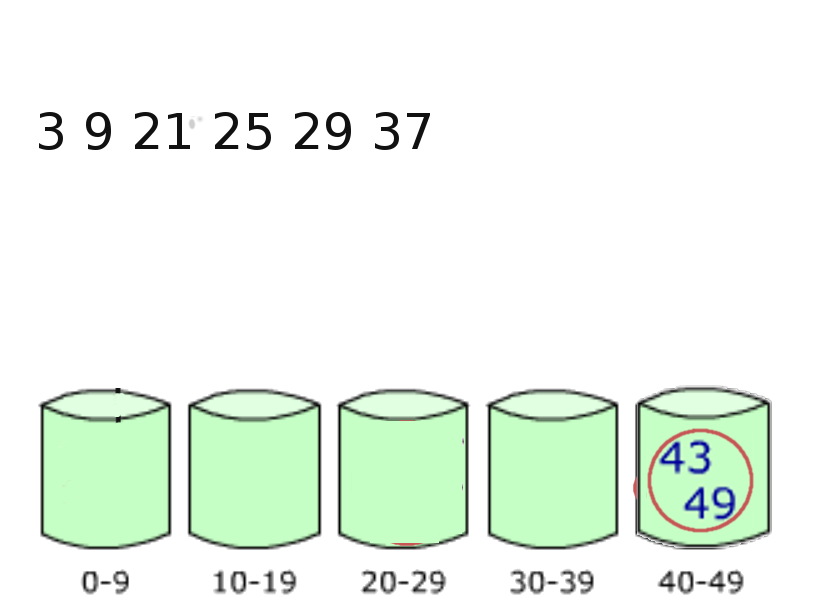
\includegraphics[scale=.3]{Figure/20.png}
	\end{figure}	
\end{frame}
\begin{frame}
	\frametitle{Sorting...}
	\begin{figure}
		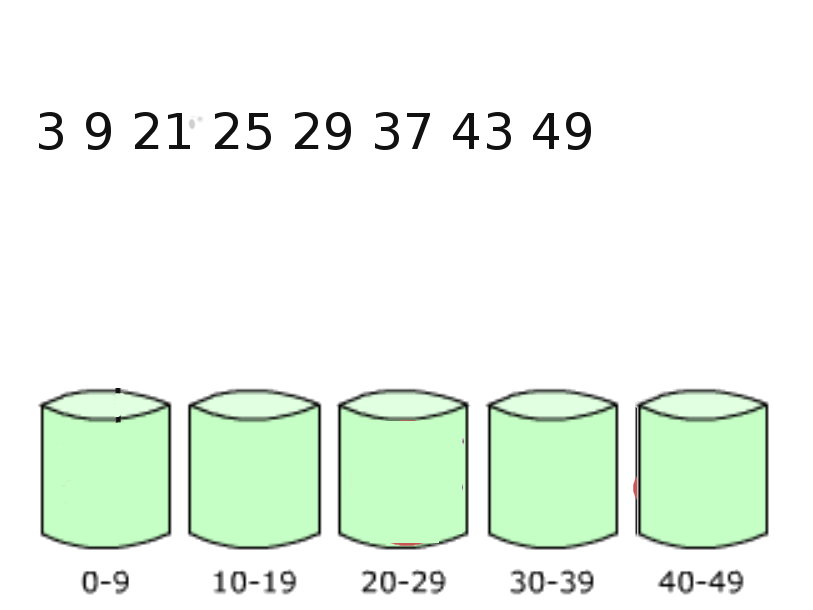
\includegraphics[scale=.3]{Figure/21.png}
	\end{figure}	
\end{frame}
\begin{frame}
	\frametitle{Sorting...}
	\begin{figure}
		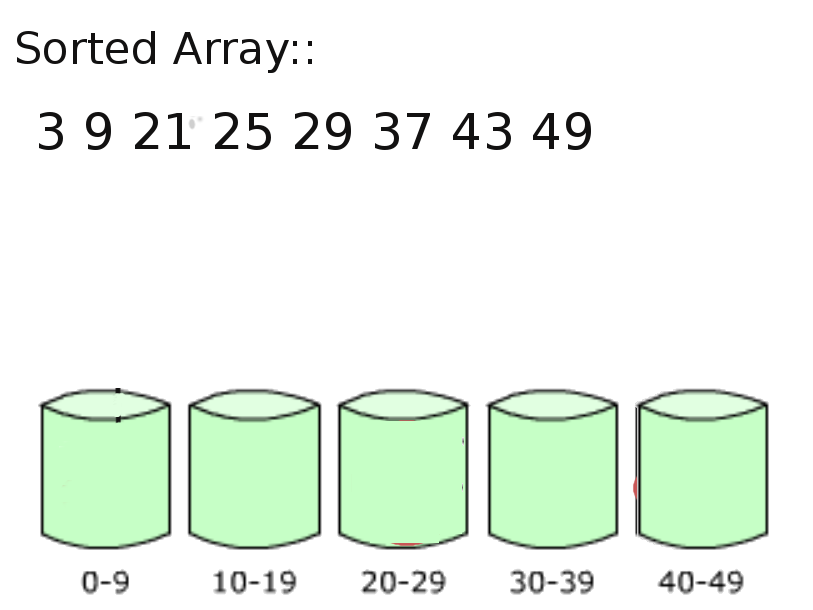
\includegraphics[scale=.3]{Figure/22.png}
	\end{figure}	
\end{frame}

\begin{frame}
	\frametitle{Implementation.}
	%While implementing the algorithm. We need:
	\begin{itemize}
		\pause
		\item Take an array of linked list.
		\pause	
		\item Each element of the array will work as a bucket.
		\pause		
		\item Put each number into the right bucket.
		\pause		
		\item Do insertion sort while putting each number.
		\pause		
		\item Merge the buckets.
	\end{itemize}
\end{frame}

\begin{frame}
	
\end{frame}
\end{document}
